\documentclass[a4paper,12pt,twoside]{memoir}

\usepackage{longtable}
\usepackage{btp}    % Use the trainermanual package option (i.e. \usepackage[trainermanual]{btp}) to generate the Trainer's version of the manual
%\usepackage[
%  noinfo,
%  cam,
%  cross,                % crosses as marks
%  a4,
%  width=6.25in,         % the width of the galley
%  height=9.25in,        % the height of the galley
%  center                % actual page is centered on the galley
%]{crop}
% Set some Workshop specific info

%\usepackage{underscore}

\usepackage{graphicx}
\usepackage{hyperref}
\usepackage{color}
\definecolor{light-blue}{rgb}{0.8,0.85,1}


\setWorkshopTitle{Introduction to Linux for Phoenix Users}
\setWorkshopVenue{University of Adelaide}
\setWorkshopDate{26th September, 2017}
\setWorkshopAuthor{
Steve Pederson\\
Stephen Bent\\
Dan Kortschak\\
Ramona Rogers\\
Robert Qiao\\
Bowen Chen\\
Exequiel Sepulveda\\
}
\begin{document}

%
% Workshop Title Page
%
\workshoptitlepage

%
% CC-BY
%
\input{licences/licence.tex}
\clearpage

\tableofcontents

\chapter{Workshop Information}
\clearpage

%
% Workshop Preamble
%
\section{The Trainers}

\newlength{\trainerIconWidth}
\setlength{\trainerIconWidth}{2.0cm}

\begin{center}
\begin{longtable}{>{\centering\arraybackslash} m{1.1\trainerIconWidth} m{1\textwidth}}

    &
    \textbf{Ms Ramona Rogers}\newline
    Computing Officer\newline
    IT Support\newline
    The University of Adelaide\newline
    South Australia\newline
    \mailto{ramona.rogers@adelaide.edu.au}\\
    \\
    &
    \textbf{Mr Robert Qiao}\newline
    Phoenix Support Team\newline
    The University of Adelaide\newline
    South Australia\newline
    \mailto{robert.qiao@adelaide.edu.au}\\
    \\
    &
    \textbf{Mr Bowen Chen}\newline
    Phoenix Support Team\newline
    The University of Adelaide\newline
    South Australia\newline
    \mailto{bowen.chen@adelaide.edu.au}\\
    \\
    &
    \textbf{Mr Exequiel Sep\'ulveda}\newline
    Phoenix Support Team\newline
    The University of Adelaide\newline
    South Australia\newline
    \mailto{exequiel.sepulvedaescobedo@adelaide.edu.au}\\
    \\
  
\end{longtable}
\end{center}


%
% Start: General Information describing the workshop and the structure of the handouts
%
\newpage
\section{Welcome}
Thank you for your attendance \& welcome to the Introduction to Linux for Phoenix Users Workshop.
This is an offering by the University of Adelaide, Reserach Computing team which is a centrally funded initiative, with the aim of assisting \& enabling researchers in their work.

This workshop is largaly based on the "Introduction to Linux" workshop deliveried by The Bioinformatics Hub. The Hub has a web-page at \url{http://www.adelaide.edu.au/bioinformatics-hub/}, and \textbf{to be kept up to date on upcoming events and workshops, please join the internal Bioinformatics mailing list on}
\url{http://list.adelaide.edu.au/mailman/listinfo/bioinfo}.\\

Phoenix has two main sources of information: \url{http://www.adelaide.edu.au/phoenix/} and or wiki page: \url{https://wiki.adelaide.edu.au/hpc/index.php/Main_Page}. \\

Phoenix team has an active Slack team for discussing questions with the local community.
Slack teams do require an invitation to join, so please email us the Hub on \mailto{hpcsupport@adelaide.edu.au} to join the community.
All are welcome.\\

Today's workshop has been put together based on previous material and courses prepared by Dr Stephen Bent (\textit{University of Queensland}), with generous technical support \& advice provided by Dr Nathan Watson-Haigh (\textit{ACPFG}) and Dr Dan Kortschak (\textit{Adelaide University, Adelson Research Group}) and complemented by Phoenix team: Ramona Rogers, Robert Qiao, Bowen Chen and Exequiel Sepulveda. 

We hope it will be useful in enabling you to continue and to advance your research.\\

\section{Course Summary}
In today's workshop, the morning session will be spent introducing you to the basic tools and concepts required for data handling.
In the afternoon session we'll develop these skills to a more advanced level, with progress in both sessions being made at your own pace.
Some people may finish early today, but the majority of you probably won't.

You will use Phoenix all the time. \\

The majority of data handling and analysis required for research uses the \textit{command line}, alternatively known as the terminal or the \textit{bash shell}.
This is a text-based interface in which commands must be typed, as opposed to the Graphical User Interfaces (aka GUIs) that most of us have become accustomed to.
Being able to access your computer using these tools enables you to more fully utilise the power \& capabilities of your machine, for both Linux \& Mac operating systems, and to a lesser extent will even enable you to dig deeper on a Windows system.\\

Whilst some of the tools we cover today may appear trivial, they are used on a daily basis by those working in the field.
These basic tools are essential for writing what are known as \textit{shell scripts}, which we will begin to cover in the afternoon session.
These are essentially simple programs that utilise the inbuilt functions of the shell, and are used to automate processes such as de-multiplexing read libraries, or aligning reads to the genome.
A knowledge of this simple type of programming and navigation is also essential for accessing the high-performance computing resources such as \texttt{phoenix}.\\

\section{Using the Post-it Notes}
For today's session, you will be provided with 3 post-it notes of differing colours.
Please use these to signal whether you need help or not by placing them on your monitors.
We will interpret these as:
\begin{enumerate}
	\item \textbf{Red} - Help! I can't make something work
	\item \textbf{Yellow} - I'm working on something, but haven't made it yet
	\item \textbf{Green} - I've finished the task I was working on
\end{enumerate}

\section{Providing Feedback}
While we endeavour to deliver a workshop with quality content and documentation in a venue conducive to an exciting, well run hands-on workshop with a bunch of knowledgeable and likable
trainers, we know there are things we could do better.

Whilst we want to know what didn't quite hit the mark for you, what would be most helpful and least
depressing, would be for you to provide ways to improve the workshop. i.e. constructive feedback.
After all, if we knew something wasn't going to work, we wouldn't have done it or put it into the
workshop in the first place!

Clearly, we also want to know what we did well! This gives us that ``feel good'' factor which will see us through those long days and nights in the lead up to such hands-on workshops!
%
%With that in mind, we'll provide some really high-tech mechanisms through which you
%can provide anonymous feedback during the workshop:
%\begin{enumerate}
%%  \item A sheet of paper, from a flip-chart, sporting a ``happy'' face and a ``not so happy'' face.
%%  Armed with a stack of colourful post-it notes, your mission is to see how many comments you can
%%  stick on the ``happy'' side!
%  
%%  \item Some empty ruled pages at the back of this handout. Use them for your own personal notes or
%%  for writing specific comments/feedback about the workshop as it progresses.
%  
%  \item An online post-workshop evaluation survey. We'll ask you to complete this before you leave.
%  If you've used the blank pages at the back of this handout to make feedback notes, you'll be able
%  to provide more specific and helpful feedback with the least amount of brain-drain!
%  
%\end{enumerate}

\section{Document Structure}
We have provided you with an electronic copy of the workshop's hands-on tutorial documents.
We have done this for two reasons: 1) you will have something to take away with you at the 
end of the workshop, and 2) you can save time (mis)typing commands on the command line by using
copy-and-paste.

\emph{We advise you to use Acrobat Reader to view the PDF. This is because it properly supports some features we have implemented to ensure that copy-and-paste of commands works as expected. This includes the appropriate copy-and-paste of special characters like tilde and hyphens as well as skipping line numbers for easy copy-and-past of whole code blocks.}\\
\\

\begin{warning}
While you could fly through the hands-on sessions doing copy-and-paste, you will learn more if you
use the time saved from not having to type all those commands, to understand what each command is
doing!
\end{warning}

The commands to enter at a terminal look something like this:
\begin{lstlisting}
tophat --solexa-quals -g 2 --library-type fr-unstranded -j annotation/Danio_rerio.Zv9.66.spliceSites -o tophat/ZV9_2cells genome/ZV9 data/2cells_1.fastq data/2cells_2.fastq
\end{lstlisting}  

The following styled code is not to be entered at a terminal, it is simply to show you the syntax of the command. 
You must use your own judgement to substitute in the correct arguments, options, filenames etc

\begin{lstlisting}[style=command_syntax]
tophat [options]* <index_base> <reads_1> <reads_2>
\end{lstlisting}

% The following is an example of how R commands are styled:

%\begin{lstlisting}[style=R]
%R --no-save
%library(plotrix) 
%data <- read.table("run_25/stats.txt", header=TRUE) 
%weighted.hist(data$short1_cov+data$short2_cov, data$lgth, breaks=0:70)
%q()
%\end{lstlisting}

The following icons are used in the margin, throughout the documentation to help you navigate around
the document more easily:

% TODO limit the use of some icons throughout as some are clearly overused and confuse the eye
\hspace*{.2cm}\vcent{\includegraphics[height=1cm]{icons/info.png}} Important\\
\hspace*{.2cm}\vcent{\includegraphics[height=1cm]{icons/notes.png}} For reference\\
\hspace*{.2cm}\vcent{\includegraphics[height=1cm]{icons/steps.png}} Follow these steps\\
\hspace*{.2cm}\vcent{\includegraphics[height=1cm]{icons/questions.png}} Questions to answer\\
\hspace*{.2cm}\vcent{\includegraphics[height=1cm]{icons/warning.png}} Warning - STOP and read\\
\hspace*{.2cm}\vcent{\includegraphics[height=1cm]{icons/bonus1.png}} Bonus exercise for fast learners\\
\hspace*{.2cm}\vcent{\includegraphics[height=1cm]{icons/bonus2.png}} Advanced exercise for super-fast learners\\


\clearpage
\section{Computer Setup}
\begin{information}
We will all be working on \texttt{Phoenix} directly, which is the University of Adelaide's High Performance Computing (HPC) system.
The software client \texttt{Bitvise} or \texttt{putty} which you will have already installed, enables us to access these machines in a familiar Desktop style, even though the majority of our time will be spent within the terminal. \\
\end{information}

\begin{warning}
In case you need to install Bitvise, download the installer from here: 
\href{https://www.bitvise.com/ssh-client-download}{Bitvise SSH Client}
\end{warning}

You will need to open a SSH session to \texttt{phoenix}.
First, we need to create a session with the basic parameters
\begin{enumerate}
	\item Hostname phoenix.adelaide.edu.au
	\item Username your student or staff ID
\end{enumerate}

Now we have created the session, you will be asked for your password. \\

\begin{note}
Now that you are connected, you will notice we are now in the head node of \texttt{Phoenix}. \\
Welcome to \texttt{Phoenix}.
\end{note}



%
% Start of modules
% Switch chapter styling to module
%
\chapterstyle{module}

\setModuleTitle{Introduction to Linux Operating System}
\setModuleAuthors{%
  Ramona Rogers, Research Services, University of Adelaide \mailto{ramona.rogers@adelaide.edu.au}\\
}
\setModuleContributions{%
  Exequiel Sepulveda, Research Services, University of Adelaide \mailto{exequiel.sepulvedaescobedo@adelaide.edu.au} \\
}

%----------------------------------------------------------------------------------------
% MODULE TITLE PAGE
%----------------------------------------------------------------------------------------
% BEGIN: Module Title Page
%  * The chapter page will always appear on odd numbered page
\chapter{\moduleTitle}

Linux has become the most used operating system for servers, and for High Performance Computing (HPC) in particular. That is the motivation to bring you this workshop.
The main goal is to show what a Linux OS is and how to use it, focus on Phoenix, the HPC facilities for supercomputing at The University of Adelaide.

\section{Components of the Linux Operating System}

An operating system is a dedicated computer program whose primary purpose is to execute other programs, to manage the hardware and system resources for those programs.
The operating system sits on top of the hardware and it is on what the general programs run.
\\
You probably are familiarised with Windows operating system, but there are many others, among the most popular are: Linux, macOS and Android.
\\
Phoenix uses Linux as operating system.
\\
The Linux operating system can be depicted as a series of layers as hardware, device-drivers, kernel, shells and special applications.

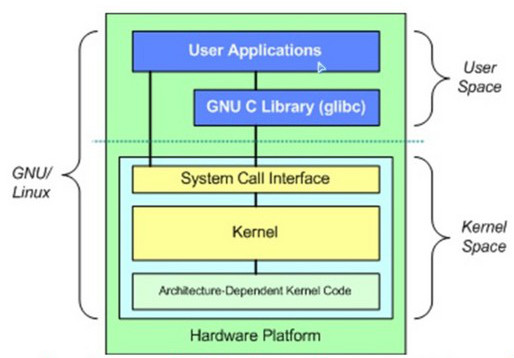
\includegraphics{linux_components}

\subsection{Hardware}
In our case the hardware are the parts of the computer like:
\begin{itemize}
\item Central processing unit or CPU. The CPU executes programs, which are located in the memory. Modern CPU has many cores enabling a first layer of parallelism.
\item Random access memory, in short RAM or memory. 
The memory allows fast access to the instructions and data that the CPU needs and because the RAM is limited it will store only information for immediate use.
Permanent data is kept in auxiliary storage on devices of the input/output subsystem.
\item Input/output subsystem contains devices called peripherals that provide input and output for the system as well as the user, and short-term and long-term storage for the processes and data. 
These devices include among others:
\begin{itemize}
\item Hard disk(s)
\item Various added cards (ie video, sound, USB-ports)
\item Monitor(s)
\item Keyboard and mouse
\item Network
\end{itemize}
\end{itemize}

On Phoenix the most relevant parts and devices are: Hard disks, RAM, Cores (CPU) and network.

\subsection{Device drivers}

Device drivers are special software used to communicate with peripheral devices.
They are called kernel modules and are usually located in one of the subdirectories of kernel.
When the device is requested the module is loaded otherwise is not. \\

The Kernel it is a small program, which is the main part of the operating system and is responsible for controlling system resources.
It is compiled from source files, object files and configurable parameters.
The kernel it is loaded into memory at very early stage when the system boots and initialised. 
Once the initialization is completed and various system daemons (processes performing system functions) have been created and made executable, the kernel waits for requests:
\begin{itemize}
\item user programs requesting services from the kernel through system calls.
\item hardware devices getting kernel response through interrupts.
\item when programs are running, the operating system creates a process to handle it.
\end{itemize} 

\subsection{Shell}
Shells are commandline language interpreters that execute commands from the standard input device (keyboard) or from file(s).
The shell is the way to interface or communicate with the operating system. 
\\
The most popular shell today is the Bourne Again Shell (BASH, originates from Born shell used in the old unix systems, called sh). There are other types like: 
csh, tcsh and ksh among others. The most used shell on Phoenix is bash.

\subsection{Programs and Applications}
Finally, the last layer is the programs and applications, which are used by users and the shell through the kernel commands to generate output or results.
A program is an executable file, and a process is an instance of the program in execution. 

\subsection{Linux accounts}
In Linux, there are three types of accounts and all are using the programs available in the operating system based on their access and rights to the system:
\begin{itemize}
\item The root account is also called superuser, which has complete and unrestricted access to the system.
Which means can run any commands but can also do big problems. On Phoenix, only administrators have root provileges.
\item The system accounts are those accounts used for the operation of the system-specific components for example mail, database and secure shell daemon accounts. These accounts are usually needed for specific functions in the system and modifying them can affect the integrity or stability of the system.
\item User accounts provide interactive access to the system for users and groups of users. 
Generally, users are assigned to this category of accounts and normally have limited access to critical system files and directories to protect the system, nevertheless,
users have full privileges to their folders and files.
\end{itemize} 

\subsection{Graphical User Interface}
Windows OS users are very familiarised with GUI and it is for sure, the most critial difference with Linux, and Phoenix in particular. 

Despite most Linux distributions has a GUI, Phoenix, as most of HPC facilities, does not support GUI. Therefore, all interaction within Phoenix must be done using a terminal.
There are many terminal programs for Windows OS, such as Putty and Bitvise. All Unix based OS (macOS and Linux) already have a terminal program to access any Linux system.

\subsection{Filesystems}
Linux OS data is organised in a folder structure, where the root folder is "/". Under this folder many subfolders are organised to support the system.
Any folder can be a physical storage unit (hard disk) or a network storage.
Examples of common subfolders of a Linux OS:
\begin{itemize}
\item /usr for common files and executables shared among users
\item /etc system configurations
\item /shared for shared resources among system and users
\item /home the parent folder of users local folders
\end{itemize} 

Phoenix has specific folders:
\begin{itemize}
\item /apps where applications and modules are installed
\item /fast where parallel storage for user are located
\item /data similar to fast but shared by users
\end{itemize} 


Any file or folder has three levels of access. The owner, the group and others.
On Phoenix, by default, any file or folder created by a user will have full permissions to its owner and no permissions for users in the same group or to any other users.
If you want to change the access to any file or folder, you need to grant explicitly.

\begin{warning}
{\Huge Don't Panic!!!}\\
More details will come in the next chapters about the practical use of the Filesystem.
\end{warning}

\setModuleTitle{Understanding file system on Phoenix}
\setModuleAuthors{%
  Bowen Chen, Technology Service, University of Adelaide\\
   \mailto{bowen.chen@adelaide.edu.au}\\
}
\setModuleContributions{%
  Bowen Chen, Technology Service, University of Adelaide\\
   \mailto{bowen.chen@adelaide.edu.au} \\
}

%----------------------------------------------------------------------------------------
% MODULE TITLE PAGE
%----------------------------------------------------------------------------------------
% BEGIN: Module Title Page
%  * The chapter page will always appear on odd numbered page
\chapter{\moduleTitle}
\newpage

\section{Home directory}
%We can display a line of text in \texttt{stdout} by using the command \texttt{echo}.
%The most simple function that people learn to write in most languages is called \texttt{Hello World} and we'll do the same thing today.
On Linux, each user has a personal directory, i.e. home directory, to store his own files and data, as well as directories. 
Your home directory on Phoenix is located at /home/$\langle$userid$\rangle$. Here, /$\langle$userid$\rangle$ means aXXXXXXX, your id.\\  \\
When you login to Phoenix, your user shell is located in your home directory. The absolute pathname of your home directory, i.e. /home/$\langle$userid$\rangle$, is also stored in the environmental variable, \$HOME. Tilde symbol, $\mathtt{\sim}$, also represent your home directory. You can use following commands to change into your home directory.
\begin{steps}
\lstset{
	literate={~} {$\sim$}{1}
	}
\begin{lstlisting}
cd ~
cd $HOME
cd /home/<userid>
\end{lstlisting}
\end{steps}

\begin{information}
%There are a few subtleties about text which are worth noting.
%Inspect the \texttt{man echo} page \& note the effects of the \texttt{-e} option.
%This allows you to specify tabs, new lines \& other special characters by using the backslash to signify these characters.
%This is an important concept \& the use of a backslash to ``escape'' normal meaning of a character is very common.
%In the following, we are using the backslash to escape the normal meanings of the \texttt{t} and \texttt{n} characters, and they can take on their ``special" meaning, such as a \texttt{tab} delimiter, or a newline.
%Try the following three commands \& see what effects these special characters have.
The /home file system is backed up, and is solely intended for the files that define your user environment and irrecoverable data such as source code. The default quota of your home directory is 10 GB.
\end{information}
\begin{information}
Don't use \$HOME for launching jobs or active job data. The /home file system hardware is not designed to support the intensive file access generated by the many hundreds of jobs that run on the Phoenix compute cores, you should use the /fast file system for job input/output instead.
\end{information}

\section{Fast directory}
The /fast directory is designed to improve the data handling performance. It is supported by high performance Lustre filesystem and is intended for active job data and immediate data storage. \\
\begin{information}
%A very common process in the command line is to take the output of one process and send it to another.
%For example, we might want to cut a column from a csv file with categorical information, and then send that field to have the different categories counted by another tool.
%This is where the concept of \texttt{stdout} becomes more important. \\
The /fast directory can handle the intensive file access created by the compute jobs that run on Phoenix. It is designed to launch jobs and store personal/research data. The default quota of your fast directory is 4 TB. \\
\end{information}
Your personal fast directory is located at /fast/users/$\langle$userid$\rangle$
The absolute pathname of your fast directory is also stored in the environmental variable, \$FASTDIR
A symbolic link to that directory can be found in your home directory, i.e. $\mathtt{\sim}$/fastdir.
Thus, you can use following commands to change into your fast directory:
\begin{steps}
\lstset{
	literate={~} {$\sim$}{1}
	}
\begin{lstlisting}
cd ~/fastdir
cd $FASTDIR
cd /fast/users/<userid>
\end{lstlisting}
\end{steps}

\begin{figure}[ht]
	\centering
	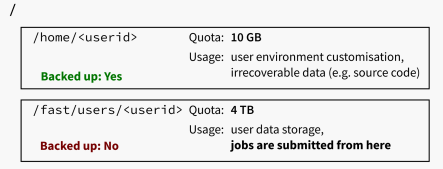
\includegraphics[width=0.9\linewidth]{images/homeFast.png} 
	\caption{Home and fast directory on Phoenix}
\end{figure}

%\begin{steps}
%By default, most command-line tools print their output to \texttt{stdout} but instead, we can send this to another tool using the pipe (\texttt{|}) symbol.
%This is exactly like putting a pipe on the output of one process, and routing it to the \textit{standard input} or \texttt{stdin} of another.
%We can use this to build up a series or chain of processes in a single line.
%A slightly ridiculous example might be to print lines 96 to 100 of the file \texttt{words} by combining \texttt{head} and \texttt{tail}
%\begin{lstlisting}
%head -n100 ~/firstname/words | tail -n5
%\end{lstlisting}
%\end{steps}

%\begin{information}
%\textbf{Note that we didn't give a file to \texttt{tail} to work with in the above command.}
%It took the \texttt{stdout} from the command \texttt{head} as it's input via \texttt{stdin}.
%This is how the pipe will work on virtually all occasions.
%\end{information}

%\begin{steps}
%As another simple example, we could take some long output from the \texttt{ls} command \& send it to the pager \texttt{less}.
%\begin{lstlisting}
%ls -lh /usr/bin | less
%\end{lstlisting}
%Page through the output until you get bored, then hit \texttt{q} to quit.
%\end{steps}

\section{Mounting filesystems}
\begin{information}
%So far, the only output we have seen has been in the terminal, i.e  \texttt{stdout}.
%Similar to the pipe command, we can redirect the output of a command \textbf{to a file} instead of \texttt{stdout}, and we do this using the greater than symbol (\textgreater), which we can almost envisage as an arrow.\\
"A file system or filesystem is used to control how data is stored and retrieved. Without a file system, information placed in a storage medium would be one large body of data with no way to tell where one piece of information stops and the next begins. By separating the data into pieces and giving each piece a name, the information is easily isolated and identified." (Wikipedia)
Mounting a filesystem simply means making the particular filesystem accessible at a certain point in the Linux directory tree.
\end{information}

\begin{steps}
You can use following commands to observe the mounting point and other information about /home and /fast on Phoenix
\end{steps}
\begin{lstlisting}
mount | egrep home
mount | egrep fast
\end{lstlisting}

%\begin{information}
%This is similar to the $>>$ trick we used earlier, but using only a single $>$ symbol will directly overwrite any existing file with the new information.
%\textbf{When using the command line, there is no }\texttt{Undo} \textbf{command.}
%Once we do something, it cannot be undone!
%\end{information}

%Once you've had a quick look at the file, exit the less pager and delete the file using the \texttt{rm} command.
%\begin{lstlisting}
%rm ampleEndings.txt
%\end{lstlisting}

\section{File and folder permissions}
Since Linux is a multi-user OS that is based on concepts of file ownership and permissions to provide security, at the file system level. Using the command, chmod, can help us to change permissions if you are the owner of the files or directories.\\
Before to use it, you need to remember several symbols and letters with the chmod. \\
\\
Identities
\begin{itemize}
\item u - the user who owns the file, i.e. owner.
\item g - the group to which the user belongs, i.e. group
\item o - others (not the owner nor the owner's group)
\item a - everyone or all (u, g, and o)
\end{itemize}

Permissions
\begin{itemize}
\item r - read access
\item w - write access
\item x - execute access
\end{itemize}

Actions
\begin{itemize}
\item + - adds the permission
\item - - removes the permission
\item = - makes it the only permission
\end{itemize}

\begin{steps}
The first thing we need to do is to create the file, foo.txt.
Use the following commands to create the file and show its default permission.
\begin{lstlisting}
touch foo.txt
ls -l foo.txt
\end{lstlisting}
When using ls -l command, you can see some thing like this: \\
-rw-r--r-- 1 a1695820 CATS\_STUDENTS 5 Sep 26 14:34 foo.txt\\
\\
Let's focus on -rw-r--r--. To explain it, parentheses will be added.\\ In -(rw-)(r--)(r--), the first pair of parentheses means the users's permission; the second means the group's permissions; the last is for all the others.\\
\\
Then using the echo command to write some words.
\begin{lstlisting}
echo "On my way to supercomputing" > foo.txt
\end{lstlisting}
Using the following command to change permissions and show current permission of it. By typing u-r, you are going to remove read permission for the user, i.e. owner, and group from the file foo.txt.
\begin{lstlisting}
chmod ug-r foo.txt
ls -l foo.txt
\end{lstlisting}
Now try to read the file with cat command
\begin{lstlisting}
cat foo.txt
\end{lstlisting}
\end{steps}

\begin{information}
When you execute commands on Phoenix, you may also meet error message like: ... Permission denied. Considering the reason caused it and how should we fix it based on what we introduced.
\end{information}

\begin{steps}
You should know what went wrong. Now let's fix the issue.
\begin{lstlisting}
ls -l foo.txt
cat foo.txt
chmod u+r foo.txt
ls -l foo.txt
cat foo.txt
\end{lstlisting}
\end{steps}

Another way to change permissions uses numeric representation.\\
Each permission setting can be represented by a numerical value:
\begin{itemize}
\item r = 4
\item w = 2
\item x = 1
\item - = 0
\end{itemize}

For example, if foo.txt has following permissions settings:\\
- (rw-) (rw-) (r--) \\
\\
Let's compute the numeric representation. The numeric representation for the user is six(4+2+0), for the group is six(4+2+0), and for others is four(4+0+0). Thus, the permissions setting is 664.\\

Bellowing is a list of common settings, numerical and meanings:
\begin{center}
	\begin{tabular}{ p{2cm}  p{3cm}  p{7cm}}
		\toprule
		\textbf{Setting} & \textbf{Numerical} & \textbf{Meaning} \\
		\midrule
		\texttt{-rw-------} & \texttt{600} & \texttt{Only owner can read and write} \\
%		\midrule
%		\texttt{.gz} & \texttt{gzip} & \texttt{gunzip} & \texttt{-d, -c, -f} \\
%								 &								& \texttt{zcat} & \\
		\midrule
		\texttt{-rw-r--r--} & \texttt{644} & \texttt{Only owner can read and write; group and others can read only} \\
		\midrule
		\texttt{-rwx------} & \texttt{700} & \texttt{Only owner can read, wirte and execute} \\
		\midrule
		\texttt{-rwxr-xr-x} & \texttt{755} & \texttt{Owner can read, wirte and execute; group and others can read and execute} \\
		\midrule
		\texttt{-rwx--x--x} & \texttt{711} & \texttt{Owner can read, wirte and execute; group and others can execute only} \\
		\midrule
		\texttt{-rw-rw-rw} & \texttt{666} & \texttt{All can read and write. (Be careful with this setting)} \\
		\midrule
		\texttt{-rwxrwxrwx} & \texttt{777} & \texttt{All can read, write and execute. (All can modify the file. Be careful.)} \\
		\bottomrule
	\end{tabular}
\end{center}

Bellowing is a list of common settings for directories:
 \begin{center}
	\begin{tabular}{ p{2cm}  p{3cm}  p{7cm}}
		\toprule
		\textbf{Setting} & \textbf{Numerical} & \textbf{Meaning} \\
		\midrule
		\texttt{-rw-------} & \texttt{600} & \texttt{Only owner can read and write in the directory} \\
		\midrule
		\texttt{-rwxr-xr-x} & \texttt{755} & \texttt{Owner can read, wirte and execute in the directory; group and others can read and execute} \\
		\bottomrule
	\end{tabular}
\end{center}


\section{Where are the applications on Phoenix?}


The applications on Phoenix are located in the /apps folder. The directory stores applications, as well as related module files. We will talk about modules on Phoenix latter.\\
%\begin{center}
%	\begin{tabular}{ p{2cm}  p{3cm}  p{3cm}   p{4cm}}
%		\toprule
%		\textbf{Suffix} & \textbf{Compress} & \textbf{Extract} & \textbf{Useful Arguments} \\
%		\midrule
%		\texttt{.zip} & \texttt{zip} & \texttt{unzip} & \texttt{-d, -c, -f} \\
%		\midrule
%		\texttt{.gz} & \texttt{gzip} & \texttt{gunzip} & \texttt{-d, -c, -f} \\
%								 &								& \texttt{zcat} & \\
%		\midrule
%		\texttt{.tar.gz} & \texttt{tar} & \texttt{tar} & \texttt{-x, -v, -f, -z} \\
%		\midrule
%		\texttt{.bz2} & \texttt{bzip2} & \texttt{bunzip2} & \\
%		\bottomrule
%	\end{tabular}
%\end{center}

%Often, files you download this way will be compressed (tar: tape archive) and archived (zipped). 
%If you see file name suffixes like .tar, .zip, .gz, and/or .bz2, among others, that is what these are.  
%To explore what these command-line options do, please check the \texttt{man} pages. \\

\begin{steps}
Let's observe the /apps directory. Firstly, list the directory's permission and what are in it.
\begin{lstlisting}
ls -ld /apps
ls -l /apps
\end{lstlisting}
You should see the two directories, modules and software. Calculating the numerical permission of the two.
Second, list what are in the directory, module
\begin{lstlisting}
ls -l /apps/modules
\end{lstlisting}
Finally, list what are in the directory, software. 
\begin{lstlisting}
ls -l /apps/modules
\end{lstlisting}
If too many things are listed, using pipe with less
\begin{lstlisting}
ls -l /apps/modules | less
\end{lstlisting}
When using less, press f key for going forward and press b key for going backward. If you want to quit, press q.
\end{steps}

%\begin{questions}
%How would we now decompress (or extract) this file?\\
%\begin{answer}
%\texttt{gunzip words.gz}\\
%\end{answer}
%
%How could we have kept our compressed file, along with the decompressed output?\\
%\begin{answer}
%\texttt{gunzip -k words.gz}\\
%\end{answer}
%
%Why would we use \texttt{zcat} instead of \texttt{gunzip -c}?\\
%\begin{answer}
%It's less typing, and it's easier to read back
%\end{answer}
%\end{questions}


%\begin{steps}
%The \texttt{GFF} file has been downloaded as a compressed file using the \texttt{gzip} program so the first thing we need to do is uncompress it.
%\begin{lstlisting}
%gunzip GCF_000011985.1_ASM1198v1_genomic.gff.gz
%\end{lstlisting}
%Don't forget to use tab auto-complete!
%\end{steps}


%\begin{steps}
%The first 7 lines of this file is what we refer to as a \textit{header}, which contains important information about how the file was generated in a standardised format.
%Many file formats have these structures at the beginning but for our purposes today we don't need to use any of this information so we can move on.
%Have a look at the beginning of the file to see what it looks like.
%\end{steps}
%\begin{lstlisting}
%head GCF_000011985.1_ASM1198v1_genomic.gff
%\end{lstlisting}

%This file begins with a few lines of header information which begin with one or two hash symbols.
%These lines contain helpful information about how the file was generated.
%The remainder of the file contains information about the genomic features themselves, in tab-separated format.
%Each line represents a genomic feature, and the tab-separated values correspond to columns in a spreadsheet.
%The first feature is annotated as a \textit{region} in the third field, whilst the second feature is annotated as a \textit{gene}.
%We'll come back to this file in the next section.
%

\setModuleTitle{Regular Expressions}
\setModuleAuthors{%
  Stephen Bent, Robinson Research Institute, University of Adelaide\\
  Steve Pederson, Bioinformatics Hub, University of Adelaide \mailto{stephen.pederson@adelaide.edu.au}\\
}
\setModuleContributions{%
  Dan Kortschak, Adelson Research Group, University of Adelaide \mailto{dan.kortschak@adelaide.edu.au} \\
  Bowen Chen, Technology Service, University of Adelaide 
  \mailto{bowen.chen@adelaide.edu.au} \\
}

%----------------------------------------------------------------------------------------
% MODULE TITLE PAGE
%----------------------------------------------------------------------------------------
% BEGIN: Module Title Page
%  * The chapter page will always appear on odd numbered page
\chapter{\moduleTitle}
\newpage

\section{Introduction}
\textit{Regular expressions} are a powerful \& flexible way of searching for text strings amongst a large document or file.
Most of us are familiar with searching for a word within a file using software such as MS Word or Excel, but regular expressions allow us to search for these with more power and flexibility, particularly in Linux files and directories management.
Instead of searching strictly for a word or text string, we can search using less strict matching criteria.
For example, we could search for a string that is either \texttt{slurm-3725} or \texttt{slurm-3825} by using the patterns  \texttt{slurm-3[78]25} or  \texttt{slurm-3(7|8)25}.
These two patterns will search for an  \texttt{slurm-3}, followed by either a  \texttt{7} or  \texttt{8}, then followed strictly by a  \texttt{25}.
Similarly a match to \texttt{slurm-37725} can be found by using the patterns \texttt{slurm-3[78][78]25} or  \texttt{slurm-3[78]\{2\}25}. \\

Whilst the bash shell has a great capacity for searching a file to matches to regular expressions, this is where languages like \textit{perl} and \textit{python} offer a great degree more power, such as more complex data structure, object-oriented programming(OOP) and more libraries.
%The commands \texttt{awk} \& \texttt{sed} which we will look at later today also use regular expressions to great effect.

%This type of searching is also very common for matching sample names, or extracting key pieces of information from master sample sheets.

\section{The command \texttt{grep}}
The built-in command which searches using regular expressions in the terminal is \texttt{grep}.
This function searches a file or input on a line-by-line basis, making patterns split across lines more difficult to find, which is one place that a programming language like Python or Perl would become preferable.  
The \texttt{man grep} page contains more detail on regular expressions under the \texttt{REGULAR EXPRESSIONS} header (scroll down a few pages).  
As can be seen in the \texttt{man} page, the command follows the form
\begin{lstlisting}[style=command_syntax]
grep [OPTIONS] 'pattern' filename
\end{lstlisting}
The option \texttt{-E} is preferable as it stands for Extended, which we can think of as ``Easier''.
As well as the series of conventional numbers and characters that we are familiar with, we can match to characters with special meaning, as we saw above where enclosing the two letters in brackets gave the option of matching either. 
The \texttt{-E} option opens up the full set of wild-card characters, and can also be called simply by using \texttt{egrep} instead of \texttt{grep -E}.
This is the default version that many of us use.\\

\begin{center}
\renewcommand{\arraystretch}{1.6}
\begin{tabular}{|p{4cm} | p{11.cm} |}
\hline
Special Character & Meaning \\ \hline
\textbackslash w & match any letter or digit, i.e. a word character \\
\textbackslash s & match any white space character, includes spaces,
tabs \& end-of-line marks \\
\textbackslash d & match any digit from 0 to 9 \\
. & matches any single character \\
+ & matches one or more of the preceding character (or pattern) \\
\** & matches zero or more of the preceding character (or pattern) \\
? & matches zero or one of the preceding character (or pattern) \\
\{x\} or \{x,y\} & matches x or between x and y instances of the preceding
character \\
\^{} & matches the beginning of a line (when not inside square brackets) \\
\$ & matches the end of a line \\
() & contents of the parentheses treated as a single pattern \\
{[}] & matches any one of the characters inside the brackets \\
{[}\^{}] & matches anything other than any of the characters in the brackets \\
\texttt{|} & either the string before or the string after the "pipe" (use parentheses) \\
\textbackslash & don't treat the following character in the way you normally would. This is why the first three entries in this table started with a backslash, as this gives them their ``special'' properties, whereas placing a backslash before a `.' symbol will enable it to function as an actual dot/full-stop. \\
\hline
\end{tabular}
\end{center}

\section{Pattern Searching}
In this section we'll learn the basics of using the \texttt{egrep} command \& what forms the output can take.
%In your \texttt{\~{}/firstname/} directory you can find the file \texttt{words}, which we placed there earlier today.
Using the command to download the file, regular\_express.txt
\begin{lstlisting}[style=command_syntax]
cp /apps/examples/training_linux/regular_express.txt .
\end{lstlisting}

This is simply a text file with several words on every line. \\

\begin{steps}
Make sure the txt file in your working directory  or else \texttt{egrep} won't be able to find the file. \\

Now let's try a few searches to get a feel for the basic syntax of the command.
Using the previous table of special characters, try to describe what you're searching for on your notes \textbf{BEFORE} you enter the command.
Do the results correspond with what you expected to see?

\begin{lstlisting}
egrep -n 't[ae]st' regular_express.txt
\end{lstlisting}
\begin{lstlisting}
egrep -n 'oo' regular_express.txt
\end{lstlisting}
\begin{lstlisting}
egrep -n '[^g]oo' regular_express.txt
\end{lstlisting}
\begin{lstlisting}
egrep -n '[^a-z]oo' regular_express.txt
\end{lstlisting}
\begin{lstlisting}
egrep -n '[0-9]' regular_express.txt
\end{lstlisting}
\begin{lstlisting}
egrep -n '[^[:lower:]]oo' regular_express.txt
\end{lstlisting}
\begin{lstlisting}
egrep -n '^[a-z]' regular_express.txt
\end{lstlisting}
\end{steps}

\begin{steps}
In the above, we were changing the pattern to extract different results from the files.
Now we'll try a few different options to change the output, whilst leaving the pattern unchanged.
If you're unsure about some of the options, don't forget to consult the \texttt{man} page. \\
\begin{lstlisting}
egrep -n 'the' regular_express.txt
\end{lstlisting}
\begin{lstlisting}
egrep -vn 'the' regular_express.txt
\end{lstlisting}
\begin{lstlisting}
egrep -in 'the' regular_express.txt
\end{lstlisting}
\end{steps}

%\section{A More Biological Context}
%
%\begin{steps}
%Let's return to the \texttt{GFF} file we downloaded in the previous section.
%\end{steps}
%
%\begin{questions}
%Before we use regular expressions, use a previous tool to find how many features you think are contained in this file?\\
%\begin{answer}
%\texttt{wc -l GCF\_000011985.1\_ASM1198v1\_genomic.gff} \\
%\end{answer}
%
%
%As we know, this file contains 7 header lines beginning with \texttt{\#}, and there may be more strange lines later in the file.
%Can you think of a way to count features by telling \texttt{egrep} to ignore these lines?
%You may need to check the manual.
%
%\begin{answer}
%This will give 4355, but the first 7 lines are header lines.
%To count the non-header lines you could try several things:\\
%\texttt{egrep -vc `\^{}\#' GCF\_000011985.1\_ASM1198v1\_genomic.gff} \\
%or\\
%\texttt{egrep -c `\^{}[\^{}\#]' GCF\_000011985.1\_ASM1198v1\_genomic.gff} \\
%\end{answer}
%
%\end{questions}
%
%As mentioned above, this file contains multiple features such as \textit{regions}, \textit{genes}, \textit{CDSs}, \textit{exons} or \textit{tRNAs}.
%If we wanted to find how many regions are annotated in this file we could use the processes we've learned above:
%\begin{lstlisting}
%egrep -c `region' GCF\_000011985.1\_ASM1198v1\_genomic.gff
%\end{lstlisting}
%
%If we wanted to count how many genes are annotated, the first idea we might have would be to do something similar using a search for the pattern \texttt{`gene'}. 
%
%\begin{questions}
%Do you think this is the number of genes?
%Try searching for the number of coding DNA sequences using the same approach (i.e. CDS) \& then add the two numbers?
%Is this more than the total number of features we found earlier?
%Can you think of a way around this using regular expressions?
%\begin{answer}
%Note that some of the occurrences of the word \textit{gene} appears in many lines which are not genes.
%We need to restrict the search to one of the tab-separated fields by including a white-space character in the search.
%The command:\\
%\texttt{egrep -n `.+\textbackslash s.+\textbackslash sgene\textbackslash s' GCF\_000011985.1\_ASM1198v1\_genomic.gff | wc -l} \\
%will give a much different result as now we are searching for the word gene surrounded by white-space, after at least two tab delimiters.
%\end{answer}
%
%Alternatively, there is a command \texttt{cut} available.
%Call the manual page (\texttt{man cut}) and inspect the option \texttt{-f}.
%The information about the types of features annotated is in the third field.
%Try to think of a way of searching this field alone.
%\begin{answer}
%\texttt{cut -f3 GCF\_000011985.1\_ASM1198v1\_genomic.gff | grep -c `gene'}\\
%Or even more accurately
%\texttt{cut -f3 -s GCF\_000011985.1\_ASM1198v1\_genomic.gff | egrep -c `gene'}\\
%although it gives the same results in this instance
%\end{answer}
%\end{questions}
%
%
%\begin{bonus}
%\begin{questions}
%
%A similar question may be how many \textit{types} of features are in this file?
%The commands \texttt{cut}, along with \texttt{sort} and \texttt{uniq} may prove to be useful when answering this.
%\begin{answer}
%\texttt{ cut -f3 -s GCF\_000011985.1\_ASM1198v1\_genomic.gff | sort | uniq | wc -l}
%\end{answer}
%
%Or we could ask how many of each type of feature are there in this file.
%\begin{answer}
%\texttt{ cut -f3 -s GCF\_000011985.1\_ASM1198v1\_genomic.gff | sort | uniq -c}
%\end{answer}
%
%\end{questions}
%\end{bonus}
%
%
%
%\section{Pattern Matching in DNA sequences}
%
%Let's try searching for some DNA patterns using a fasta file.
%We can download the genomic sequence for the same organism, so once again head to the same page as last time, but this time copy the link to the \textbf{genome}.
%
%\begin{lstlisting}
%wget <<paste address here>>
%gunzip GCF_000011985.1_ASM1198v1_genomic.fna.gz
%\end{lstlisting}
%
%Let's try using some of the tricks we've learned above.
%
%\begin{questions}
%How many times does the sequence \texttt{GAAAGGATTA} appear in the genome?\\
%\begin{answer}
%\texttt{egrep -c 'GAAAGGATTA' GCF\_000011985.1\_ASM1198v1\_genomic.fna} \\
%Gives 3\\
%\end{answer}
%How many times does this appear, but with two \textbf{or more} Ts before the final A?\\
%\begin{answer}
%\texttt{egrep -c 'GAAAGGATT+A' GCF\_000011985.1\_ASM1198v1\_genomic.fna}\\
%Gives 4\\
%\end{answer}
%How many times does this appear, but with two \textbf{or more} Ts but with a G or C following the final T?\\
%\begin{answer}
%\texttt{egrep -c 'GAAAGGATT+[\^A]' ...}
%Gives 7.
%Clearly, they could also specify (GC) instead of [\^A].
%\end{answer}
%\end{questions}


%\begin{information}
%Now we can have a look through the GBS-Seq file (\texttt{pair1.fq}) that we copied \& renamed earlier.
%Before we search the the file, we should know what we this data actually is.
%These are a small subset of 100bp reads from a GBS-Seq experiment \& are from the first sample in a set of paired reads.
%Although we can't tell this directly from this file, the sequences were obtained from a rabbit affected by \textit{calicivirus}.
%\end{information}
%
%\begin{steps}
%If you inspect the data using the \texttt{head} command, you'll notice that the file is in sets of four lines, as defined by the fastq format.
%\begin{lstlisting}
%head pair1.fq
%\end{lstlisting}
%The first line contains a \textit{sequence identifier}, the second line is the \textit{sequence} itself, the third line is simply the `+' symbol as a placeholder \& the final line is a set of characters which correspond to \textit{quality scores} for each base.
%We'll be looking at this file structure in much more detail next week, so that's all we need to know for today's session.
%\end{steps}
%
%\begin{questions}
%As these reads are from the first sample in a set of paired reads, the final value in the sequence identifier is \texttt{\_1}.
%How could we search for a pattern just to extract the sequence identifiers? \\
%\begin{answer}
%\texttt{egrep `\^{}@.+\_1\$' pair1.fq}
%\end{answer}
%
%Reads from the second in the set of paired reads would have an identifier that ends with the pattern \texttt{\_2}.
%There are no reads in the file \texttt{pair1.fq} that are the second pair, so what would you expect to see if you changed the \texttt{\_1} in the previous query to \texttt{\_2}? \\
%\begin{answer}
%If they didn't include the EOL symbol, they'll get results...
%\end{answer}
%
%\end{questions}
%
%\begin{steps}
%Now we'll try searching for some sequences, so try the following search string. 
%Does the output match what you expected? \\
%\texttt{grep -En `TGCAGGCTCT' pair1.fq}
%\end{steps}
%
%This should give lines 774, 3382, 3758, 7326, 7594 \& 9566 along with the sequence information and matching fragment highlighted in red.\\
%
%\begin{questions}
%For the following search string \\
%\texttt{grep -En `TGCAGGCTCT.+(GA)\{2\}.+A\{3\}' pair1.fq} \\
%What do the following components of the pattern match to: \\
%\texttt{`.+'} \\
%\begin{answer}
%This matches an unspecified length of any character, until the next key match is found. \\
%\end{answer}
%
%\texttt{(GA)\{2\}} \\
%\begin{answer}
%This matches to two repeats of the pattern GA. \\
%\end{answer}
%
%\texttt{A\{3\}}\\
%\begin{answer}
%This matches three `A's in a row. \\
%\end{answer}
%
%How could you find the sequence identifier for the above match?\\
%\begin{answer}
%\texttt{grep -EnC1 `TGCAGGCTCT.+(GA)\{2\}.+A\{3\}' pair1.fq} or \\
%\texttt{grep -EnB1 `TGCAGGCTCT.+(GA)\{2\}.+A\{3\}' pair1.fq}
%\end{answer}
%\end{questions}

\setModuleTitle{The Tools sed \& awk}
\setModuleAuthors{%
  Stephen Bent, Robinson Research Institute, University of Adelaide\\
  Steve Pederson, Bioinformatics Hub, University of Adelaide \mailto{stephen.pederson@adelaide.edu.au}\\
}
\setModuleContributions{%
  Dan Kortschak, Adelson Research Group, University of Adelaide \mailto{dan.kortschak@adelaide.edu.au} \\
}

%----------------------------------------------------------------------------------------
% MODULE TITLE PAGE
%----------------------------------------------------------------------------------------
% BEGIN: Module Title Page
%  * The chapter page will always appear on odd numbered page
\chapter{\moduleTitle}
\newpage

\section{sed: The Stream Editor}
\begin{information}
One very useful command in the terminal is \texttt{sed}, which is short for \textit{\underline{s}tream \underline{ed}itor}.
Instead of the \texttt{man} page for \texttt{sed} the \texttt{info sed} page is larger but a little easier to digest.
This is a very powerful command which can be a little overwhelming at first.
If using this for your own scripts \& you can't figure something out, remember ``Google is your friend'' \& sites like \url{www.stackoverflow.com} are full of people wrestling with similar problems to you.
You can be certain you're not the first person to be stumped by a problem \& these are great places to start looking for help. 
Even advanced programmers use Google \& Stack Overflow to find solutions.\\
\end{information}

For today, there are two key \texttt{sed} functionalities that we want to introduce.\\
\begin{enumerate}
\item Using \texttt{sed} to alter the contents of a file/input;
\item Using \texttt{sed} to print regions of a file
\end{enumerate}

\subsection*{Altering a file or other input}
\texttt{sed} uses \textit{regular expressions} that we have come across under the \texttt{grep} section, and we can use these to replace strings or characters within a text string.
The command works in the form 
\begin{lstlisting}[style=command_syntax]
sed SCRIPT INPUT
\end{lstlisting}
and the script section is where all the action happens.
Input can be given to \texttt{sed} as either a file, or just as a text stream via \texttt{stdin} using the \textit{pipe} symbol that we have already introduced.

\begin{steps}
In the following example the script section begins with an `s' to indicate that we are going to make a substitution.
The beginning of the first pattern (i.e. the \textit{regexp} we are searching for) is denoted with the backslash, with the identical delimiter indicating the replacement pattern, and this is in turn completed with the same delimiter.
Try this simple example from the link \url{http://www.grymoire.com/Unix/Sed.html} which is a very detailed \& helpful resource about the usage \texttt{sed}.
Here we are sending the input to the command via the pipe, so no `INPUT' section is required: \\
\end{steps}

\begin{lstlisting}
echo Sunday | sed 's/day/night/' 
\end{lstlisting}

Here you are passing \texttt{sed} the string Sunday, and \texttt{sed} takes day and turns it into night.  
\texttt{sed} will only replace the first instance of the string on any line, so try: \\

\begin{lstlisting}
echo Sundayday | sed 's/day/night/' 
\end{lstlisting}

Note that it only replaced the first instance of day and left the second.  
However, you can make it 'global', where it switches every instance by using the `g' option at the end of the pattern like this: \\

\begin{lstlisting}
echo Sundayday | sed 's/day/night/g' 
\end{lstlisting}

You can also `capture' parts of the pattern in parentheses and access that in the second part of the regular expression (what you are switching to) using \textbackslash 1, \textbackslash 2, etc., to denoted the number of the captured string, in the order they were captured.
If you want to match `ATGNNNTGA', where N is any base, and just output these three bases you could try the following:\\
\begin{lstlisting}
echo 'ATGCCAGTA' | sed -r 's/ATG(.{3})GTA/\1/g'
\end{lstlisting}

Clearly, we have just given this command a sequence so we know exactly what to expect.
However, hopefully this demonstrates the concept of extracting a subset of the sequence.

Or if we needed to replace those three bases with an expanded repeat of them, you could do the following where we capture the undefined string between \texttt{ATG} \& \texttt{GTA}, and expand it: \\
\begin{lstlisting}
echo 'ATGCCAGTA' | sed -r 's/ATG(.{3})GTA/ATG\1\1\1GTA/g'
\end{lstlisting}

The \textbackslash 1 take the contents of the first parenthesis and uses it in the substitution, even though you don't know what the bases are.
Note that the `-r' option was set for these operations, which turns on extended regular expression capabilities.
This can be a powerful tool \& multiple parentheses can also be used: \\
\begin{lstlisting}
echo 'ATGCCAGTA' | sed -r 's/(ATG)(.{3})(GTA)/\3\2\2\1/g'
\end{lstlisting}

In this last command we switched the order of the first \& last triplet, and expanded the middle unknown string twice.
Note how quickly this starts to look confusing though!
Taking care to be clear when writing these types of procedures can be an important idea when you have to go back \& re-read your code a year or two later.
(Yes this will happen a lot!!!)

\begin{information}
The use of backslashes to delineate each section of the script used by \texttt{sed} is the most common convention, but we are not restricted to it.
We could have uses any `wild-card' type character to follow the `s', such as `*' `:' or `\%' although this must be consistent across all sections of the script, and should only be used if the backslash itself is part of the search or replacement string.
\end{information}

\subsection*{Displaying a region from a file}
The command \texttt{sed} can also be used to replicate some of the functionality of the \texttt{head} \& grep commands, but with a little more power at your fingertips.
By default \texttt{sed} will print the entire input stream it receives, but setting the option `-n' will turn this off.
Try this by adding an `n' immediately after the `-r' in one of the above lines \& you will notice you receive no output.
This is useful if we wish to restrict our output to a subset of lines within a file, and by including a `p' at the end of the script section, only the section matching the results of the script will be printed.
\begin{steps}
Make sure you are in the correct directory \& we can look through the \texttt{regular\_express.txt} file again.
\begin{lstlisting}
sed -n '1,10p' regular_express.txt
\end{lstlisting}
This will print the first 10 lines, like the \texttt{head} command will by default.
However, we could now print any range of lines we choose.
Try this by changing the script to something interesting like `15,21p'.\\
\\
We could also restrict the range to specific lines by using the \texttt{sed} increment operator `\~{}'.
\begin{lstlisting}
sed -n '1~5p' regular_express.txt
\end{lstlisting}
This will print every 5th line, beginning at the first.
\end{steps}

\begin{steps}
We can also make sed operate like \texttt{grep} by making it only print the lines which match a pattern.
\begin{lstlisting}
sed -rn '/g[o]*d/ p' regular_express.txt
\end{lstlisting}
Note however, that the line numbers are not present in this output.
\end{steps}

%\begin{questions}
%How would we use \texttt{sed} to extract the lines from the genome sequence which match the pattern \texttt{ATGC.+ACAA.*}? What text does this pattern represent?\\
%\begin{answer}
%\texttt{ sed -rn '/ATGC.+ACAA.*/p' GCF\_000011985.1\_ASM1198v1\_genomic.fna}\\
%\end{answer}
%How would we use the pipe to extract the unspecified sequence between the ATGC and the ACAA?\\
%\begin{answer}
%\texttt{sed -rn '/ATGC.+ACAA.*/p' GCF\_000011985.1\_ASM1198v1\_genomic.fna | sed -r 's/ATGC(.+)ACAA.*/\textbackslash 1/g'
%}
%\end{answer}
%\end{questions}

\section{Some Important Programming Concepts}

Before moving on to awk, we need to quickly recap two of the most widely used techniques in programming:
\begin{enumerate}
  \item The \texttt{for} loop
  \item Logical tests using an \texttt{if} statement
\end{enumerate}

\subsubsection*{For Loops}

\begin{steps}
A \texttt{for} loop is what we use to cycle through an input one item at a time.
As a simple example, we could print each number from a set of numbers.
\begin{lstlisting}
for i in 1 2 3; do (echo -e $i); done
\end{lstlisting}
\end{steps}

\begin{information}
In the above code, the fragment before the semi-colon asked the program to cycle through the values 1, 2 \& 3, letting the variable `i' take each value in order of appearance.
First i = 1, then i = 2 \& finally i = 3.
If you're wondering why we chose `i', it just seemed like a sensible choice for an integer. 
We simply needed to choose a name for a \textit{variable} which we would pass the values to.\\

After assigning each value to \texttt{i}, was the instruction on what to do for each value.
Note that the value of the variable `i' was \textit{prefaced by the dollar sign (\$).
This is how the bash shell knows it is a variable, not the letter `i'.}
The command \texttt{done} then finished the \texttt{do} command.
All commands like \texttt{do}, \texttt{if} or \texttt{case} have completing statements, which respectively are \texttt{done}, \texttt{fi} \& \texttt{esac}.\\

Another important concept which was glossed over in the previous paragraph is that of a \textit{variable}.
These are essentially just `\textit{placeholders}' which have a value that can change (hence the name).
In the above loop, the same operation was performed on the variable \texttt{i}, but the value changed from 1 to 2 to 3.
Variables in shell scripts can hold numbers or text strings and don't have to be formally defined as in some other languages.
\end{information}

\begin{advanced}
An alternate approach could be to make a breathtaking claim about some files.
Here we'll use the variable called `f', which seems sensible for a filename.
\begin{lstlisting}
cd /apps/examples/training_linux/scripting/
for f in $(ls); do (echo -e "I can see the file $f"); done
cd -
\end{lstlisting}
\end{advanced}

Note, that we've also assigned the output from the command \texttt{ls} to this variable, by using the \$() syntax.
The use of double quotes for the \texttt{echo} command also allows us to refer to the values held by f.
Single quotes at this point would only return the characters `\$f'.

\subsubsection{If Statements}
If statements are those which only have a binary `yes' or `no' response, or more correctly a \texttt{TRUE}/\texttt{FALSE} response.
For example, we could specify things like:
\begin{itemize}
\item \texttt{if} (i$>1$) then \texttt{do} something, or
\item \texttt{if} (fileName==bob.txt) then \texttt{do} something else
\end{itemize}

\begin{information}
Notice that in the second if statement, there was a double equals sign.
This is the programmers way of saying \textit{compare} the first argument with the second argument.
A single equals sign is generally interpreted by a program as \textit{assign} the value of the first argument to be the second argument.
This use of `double operators' is very common, notably you will see \&\& to represent the command `\textit{and}', and $\Vert$ to represent `\textit{or}.'
A final useful trick to be aware of is the use of an exclamation mark to reverse a command.
A good example of this is the use of the command `!=' as the representation of \textit{not equal to} in a logical test.
\end{information}

\section{awk: A command and a language}
Moving on to \texttt{awk}, this is a very useful tool which can be used either as a command, as well as functioning as it's own language.
We'll just use it as a command today, and it is extremely useful for dealing with tab- or comma-separated files, such as we often see in biological data.\\
\begin{information}
The basic structure of an \texttt{awk} command is: 
\begin{lstlisting}[style=command_syntax]
awk '/<pattern>/' file
\end{lstlisting}
\texttt{awk} will then search the file and output any line containing the regular expression pattern (kind of like \texttt{grep)}.
With \texttt{awk}, you can also do: 
\begin{lstlisting}[style=command_syntax]
awk '\{<code>\}' file
\end{lstlisting}
where you can put a program, or set of instructions in the curly braces. 
In the code, you can specify values from different columns of the file by using the numbers \$1, \$2, etc., (or you can use \$0 for the whole line).
Values can also be returned in the output by using the command \texttt{print} followed by the field number.
\end{information}

\begin{steps}
We have that regular\_express.txt file and we've already looked at it at little, so let's pull out some particular features!
Make your terminal as wide as the screen, then change into the appropriate directory \& enter
\begin{lstlisting}
 awk '{if  ($3=="is")  print $0}' regular_express.txt
\end{lstlisting}
Here we've specified that the third field must be is. \\

We could make it a little more complex and just look for genes in a given region.
\textbf{In the following line, the symbol `\textbackslash ' has been placed here to indicate it is a single line, extending beyond the width of the page.
Do not enter this character!}
\begin{lstlisting}
awk '{if ( ($3=="gene") && ($4 > 10000) && ($4 < 20000) ) print $0}' regular_express.txt
\end{lstlisting}
\end{steps}
\begin{note}
In the above code, \texttt{\$3==``gene''} asks for the entry in the third field to be ``gene.''
The next two fragments request for the values in the fourth field (i.e. \$4) to be between 10000 \& 20000.
%awk '{if (($5 - $4 > 1000) && ($3 == "gene")) print $1, $2, $4, $5, $9}' regular_express.txt
Notice that each these three commands were enclosed in a pair of brackets within an outer pair of brackets.
This gave a command of the form: \\
\texttt{( (Condition1) \&\& (Condition2) \&\& (Condition3) )} \\
After this came the fragment \texttt{print \$0} which asked \texttt{awk} to print the entire line if the 3 conditions are true.
You've just written (\& hopefully understood) a computer program!
\end{note}

\begin{steps}
Another example (what does this do?): \\
\begin{lstlisting}
awk '{if (($5 - $4 > 1000) && ($3 == "gene")) print $0}' regular_express.txt
\end{lstlisting}
If you don't want to output all of the columns, you can specify which ones to output.  
While we're at it, let's save the output as a file: \\
\begin{lstlisting}
awk '{if (($5 - $4 > 1000) && ($3 == "gene")) print $1, $2, $4, $5, $9}' regular_express.txt > awkout.txt
\end{lstlisting}
\end{steps}

\begin{advanced}
The command \texttt{awk} has a pretty serious set of in-built commands which can be used in the code sections as above.
Although it looks a little overwhelming, there is a detailed page \url{http://www.grymoire.com/Unix/Awk.html} which gives a rundown on the full capabilities of the language.
One command that we may find helpful is \texttt{length}, which counts the number of characters in a line.

%In your \texttt{trainingData} directory you'll find another file \texttt{seqData.fastq}.
%This is a small set of reads from some mRNA pulled down by Immunoprecipitation, and they've been processed to have varying lengths.

%\begin{questions}
%Can you think of a way to combine \texttt{sed} and \texttt{awk} to create a new file \texttt{lengths.txt} which contains the length of every read in the file \texttt{seqData.fastq}?
%\end{questions}
%\begin{answer}}
%\texttt{sed -n `2\~{}4p' seqData.fastq | awk `\{print length(\$1)\}' > lengths.txt}
%\end{answer}
\end{advanced}

\setModuleTitle{Command Line Editors}
\setModuleAuthors{%
  Robert Qiao, Research Services Phoenix Team, University of Adelaide
\mailto{robert.qiao@adelaide.edu.au}\\ 
}

%----------------------------------------------------------------------------------------
% MODULE TITLE PAGE
%----------------------------------------------------------------------------------------
% BEGIN: Module Title Page
%  * The chapter page will always appear on odd numbered page
\chapter{\moduleTitle}
\newpage

In addition to the streaming editor named sed as you have studied earlier, which operates on a file
in a non-interactive mode according to a set of instructions that you specify on the command line or
in a
script. It can be used for "canned" editing tasks that must be applied in the same way to many
files. More commonly, we use interactive editors and there are three powerful interactive text
editors that
are commonly used on Unix computers: vi, pico, and emacs. \\

Although vi, pico, emacs are extremely powerful, to get a firm grasp takes some efforts and most of
times we just need to open, amend and save a file without remembering the keyboard shortcuts.
Luckly, there is such editor called nano and that is what we will use for the class today.
The nano editor has its own set of keyboard shortcuts of course and in this guide I aim to help you
to understand the meaning of all those special keystrokes you can use to make your life easier when
using nano. \\
But before we dive into the nano, let's generally go over some of the streamline editors like vi,
emacs. 

\section {vi}

\begin{information}
Vi (pronounced "vee-eye") is the standard editor for Unix systems. It is universally available on
Unix systems. Vi is a screen editor. It treats your computer screen as a window into the file. You
move the window around to view different parts of the file. You move the cursor to the location on
the screen where you want to make a change; or optionally, you specify some kind of global change.
Vi updates your screen to reflect changes that you make in the file. Actually, it works on a copy of
the file in memory, and only updates the file on disk when you tell it to, such as when you end the
editing session. \\
Main advantages of vi are including: 
\begin{itemize}
  \item Vi is universally available on Unix systems. It has been around so long in a stable form
that it is essentially bug free. Many clones have been written for other kinds of computers.
  \item Vi has many powerful commands that utilize just the alphanumeric keys -- it does not require
special function keys.
  \item Vi is a small program that does not require a lot of system memory or CPU time. It works
very fast, even on large files.
  \item While vi is not programmable, it has a simple way to let other Unix programs, such as the
sort utility, work on selected portions of your file. This adds the functionality of all those
programs to the editor.
  \item Vi is completely terminal device independent. It will work with any kind of terminal.
A system file describes the capabilities and control sequences of each kind of terminal for vi. All
the program needs to know is what type of terminal you have. When you log in, if pangea cannot
figure out what kind of terminal you have, it will prompt you to specify a terminal type. The most
common type is the vt100, which most modern terminals and PC communications software emulate.
\end{itemize}
\end{information} 

\setModuleTitle{Writing Scripts}
\setModuleAuthors{%
  Stephen Bent, Robinson Research Institute, University of Adelaide\\
  Steve Pederson, Bioinformatics Hub, University of Adelaide
\mailto{stephen.pederson@adelaide.edu.au}\\
  Robert Qiao, Research Services Phoenix Team, University of Adelaide
\mailto{robert.qiao@adelaide.edu.au}\\ 
}
\setModuleContributions{%
  Dan Kortschak, Adelson Research Group, University of Adelaide
\mailto{dan.kortschak@adelaide.edu.au} \\
  Jimmy Breen, Robinson Research Institute \& Bioinformatics Hub, University of Adelaide
\mailto{jimmy.breen@adelaide.edu.au}\\
}

%----------------------------------------------------------------------------------------
% MODULE TITLE PAGE
%----------------------------------------------------------------------------------------
% BEGIN: Module Title Page
%  * The chapter page will always appear on odd numbered page
\chapter{\moduleTitle}
\newpage

We often need to perform repetitive tasks, or need to perform complex series of procedures. Rather
than typing instruction receptively and stearing the screen waiting for each process to finish
before providing next instruction, writing the set of instructions into a script and interpreter/compiler 
does the waiting and stearing for us is a very powerful way of
liberating our time. They are also an excellent way of ensuring the commands you have used in your
research are retained for future reference.
Keeping copies of all electronic processes to ensure reproducibility is a very important component
of any research. 
Writing scripts requires an understanding of several key concepts which form the foundation of much
computer programming, so let's walk our way through a few of them. \\


\section{Shell Scripts}
Now that we've been through just some of the concepts \& tools we can use when writing scripts, it's
time to tackle one of our own where we can bring it all together.

\begin{information}
Every bash script begins with what is known as a \textit{shebang}, which we would commonly recognise
as a hash sign followed by an exclamation mark, i.e \texttt{\#!}.
This is immediately followed by \texttt{/bin/bash}, which tells the interpreter to run the command
\texttt{bash } in the directory \texttt{/bin}.
(This is actually where the program \texttt{bash} lives on a Linux system.)
This opening sequence is vital \& tells the computer how to respond to all of the following
commands.
As a string this looks like:\\

\texttt{\#!/bin/bash}\\
\end{information}

\begin{note}
The hash symbol generally functions as a comment character in scripts.
Sometimes we can include lines in a script to remind ourselves what we're trying to do, and we can
preface these with the hash to ensure the interpreter doesn't try to run them.
It's presence as a comment here, followed by the exclamation mark, is specifically looked for by the
interpreter but beyond this specific occurrence, comment lines are generally ignored by scripts \&
programs.
\end{note}

\subsection{Some Example Scripts}
Let's now look at some simple scripts.
These are really just examples of some useful things you can do \& may not really be the best
scripts from a technical perspective. Hopefully they give you some pointers so you can get going
\begin{warning}
To setup this part of the course, please login to your Phoenix account and download the example file to your /fastdir directory now
\begin{lstlisting}
cp -r /apps/examples/training_linux/ ~/fastdir/
\end{lstlisting}
please check to make sure you command blow contains valid 4 files. If you see error messages, please indicate to tutors, 
you should get this step fixed before carry on further
\begin{lstlisting}
ls -al ~/fastdir/training_linux
\end{lstlisting}
\end{warning}

\subsubsection*{A Simple Example to Start}
\begin{warning}
\textbf{Don't try to enter these commands directly in the terminal!!!}
They are designed to be placed in a script which we will do after we've inspected the contents of
the script.
First,  just have a look through the script \& make sure you understand what the script is doing.

Also remember that any long lines of code may be automatically broken into new lines on your page by
the `\textbackslash ' character.
We don't want to enter this character when we create our script.
Note that the line numbers on the left of the code don't change when this happens, e.g. line 9.
\end{warning}

Before we go any further, have a look at the following script.

\begin{lstlisting}[style=command_syntax]
#!/bin/bash
#
# First we'll declare some variables with some text strings
ME='Put your name here'
MESSAGE='This is your first script'

# Now well place these variables into a command to get some output
echo -e "Hello ${ME}\n${MESSAGE}\nWell Done!"
\end{lstlisting}

\begin{information}
Firstly, you may notice some lines that begin with the \# character.
These are \textit{comments} which have no impact on the execution of the script, but are written so
you can understand what you were thinking when you wrote it.
If you look at your code 6 months from now, there is a very strong chance that you won't recall
exactly what you were thinking, so these comments can be a good place just to explain something to
the future version of yourself.
There is a school of thought which says that you write code primarily for humans to read, not for
the computer to understand.
\end{information}

\begin{questions}
In the above script, there are two variables. 
Although we have initially set them to be one value, they are still variables.
What are their names? 
\begin{answer}
ME \& MESSAGE
\end{answer}
\end{questions}

\begin{steps}
First we'll create an empty file which will become our script.
We'll give it the suffix \texttt{.sh} as that is the common convention for bash scripts.
\end{steps}
\begin{lstlisting}
cd ~/firstname
touch wellDone.sh
\end{lstlisting}

\begin{steps}
Now using the text editor \textit{nano}, enter the above code into this file \textit{setting your
actual name as the ME variable},  and save it by using \texttt{Ctrl+o}, which is indicated as
\texttt{\^O} in the nano screen.\\
\end{steps}

\begin{lstlisting}
nano wellDone.sh
\end{lstlisting}

Once you're finished, you can exit the \texttt{nano} editor by hitting \texttt{Ctrl+x}.

\begin{information}

Another coding style which can be helpful is the enclosing of each variable name in curly braces
every time the value is called.
Whilst not being strictly required, this can make it easy for you to follow in the future when
you're looking back.
Variables have also been names using strictly upper-case letters.
This is another optional coding style, but can also make things clear for you as you look back
through your work.
Most command line tools use strictly lower-case names, so this is another reason the upper-case
variable names can be helpful.
\end{information}

\begin{steps}
Unfortunately, this script cannot be executed yet but we can easily enable execution of the code
inside the script.
If you recall the flags from earlier which denoted the read/write/execute permissions of a file, all
we need to do is set the execute permission for this file.
First we'll look at the files in the folder using \texttt{ls -l} and note these triplets should be
\texttt{rw-} for the user \& the group you belong to.
To make this script executable, enter the following in your terminal.
\begin{lstlisting}
cd ~/firstname
chmod +x wellDone.sh
ls -l
\end{lstlisting}
\end{steps}

\begin{steps}
Notice that the third flag in the triplet has now become an \texttt{x}.
This indicates that we can now execute the file in the terminal.
As a security measure, Linux doesn't allow you to execute a script from within the same directory so
to execute it enter the following:
\begin{lstlisting}
./wellDone.sh
\end{lstlisting}
\end{steps}

\subsubsection{Making a Small Change}

\begin{steps}
Now let's change the variable \texttt{ME} in the script to read as
\begin{lstlisting}
ME=$1
\end{lstlisting}
and save this as \texttt{wellDone2.sh}.
(You may like to create this first using \texttt{cp})
You'll now need to set the execute permission again.
\begin{lstlisting}
chmod +x wellDone2.sh
\end{lstlisting}
\end{steps}

\begin{information}
This time we have set the script to \textit{receive input from stdin} (i.e. the terminal), and we
will need to supply a value, which will then be placed in the variable \texttt{ME}.
Choose whichever random name you want and enter the following
\begin{lstlisting}
./wellDone2.sh Boris
\end{lstlisting}
\end{information}

\begin{advanced}
As you can imagine, this style of scripting can be useful for iterating over multiple objects.
A trivial example, which builds on a now familiar concept would be to try the following.
\begin{lstlisting}
for n in Boris Fred; do (./wellDone2.sh $n); done
\end{lstlisting}
\end{advanced}

%\subsubsection*{A Script That Does Something Relevant}
%\begin{lstlisting}[style=command_syntax]
%#!/bin/bash
%FILE=$1
%
%# Find all of the possible read lengths in the supplied file
%LENGTHS=$(sed -n '2~4p' ${FILE} | awk '{print length($1)}' | sort | uniq)
%
%# Print some column headings
%echo -e "Read length\tTotal Number"
%
%# Now for each possible length, count how many reads there are of that length
%for L in ${LENGTHS}
%do
%	COUNT=$(sed -n '2~4p' ${FILE} | awk '{print length($1)}' | grep -c ${L})
%	echo -e "${L}\t${COUNT}" 
%done
%\end{lstlisting}
%
%\begin{steps}
%Now use the text editor \texttt{gedit} to write this script \& save it as \texttt{findLengths.sh}
%in your home folder.
%\end{steps}
%
%\begin{note}
%Note that after the shebang, there was a variable \texttt{FILE} which took the value \texttt{\$1}.
%This means that after we call the script, we need to specify a filename to assign to the variable
%\texttt{FILE}.
%For example, we could run the script as: \\
%\texttt{./findLengths.sh \~{}/Documents/trainingData/seqData.fastq}.\\
%This would execute the remainder of the script on that file. \\
%\end{note}
%
%\begin{questions}
%Where will the script send the output to?
%\begin{answer}
%stdout.
%\end{answer}
%
%How would we write the output to a file?
%\begin{answer}
%Use the $>$ symbol to assign it to a filename
%\end{answer}
%\end{questions}
%
%\begin{steps}
%Now we can make the script executable \& run it on the file \texttt{seqData.fastq}.
%\begin{lstlisting}
%chmod +x findLengths.sh
%./findLengths.sh ~/Documents/trainingData/seqData.fastq > lengths.txt
%\end{lstlisting}
%\end{steps}
%
%\begin{questions}
%Inspect the file using \texttt{gedit}, or the \texttt{less} pager.
%Did it look like you expected? 
%Is this a tab-separated file, or a comma or space separated file?
%\end{questions}
%
%\begin{bonus}
%Try running it on the \texttt{pair1.fq} \& \texttt{pair2.fq} files.
%\begin{questions}
%Is that what you expected?
%\begin{answer}
%All the reads should have been the same length...
%\end{answer}
%\end{questions}
%\end{bonus}
%
\clearpage
\subsection*{A more complicated script}

Here's a more complicated script with some more formal procedures.
This is a script which will extract only the ProbeFeature features from the .gff file we have been working
with, and export them to a separate file.
Look through each line carefully \& write down your understanding of what each line is asking the
program to do.

\begin{lstlisting}[style=command_syntax]
#!/bin/bash
# Declare some helpful variables
FILEDIR=~/fastdir/training_linux/scripting
FILENAME=NC_015214.gff
OUTFILE=NC_015214_CDS.txt
# Make sure the directory exists
if [ -d ${FILEDIR} ]; then
	echo Changing to ${FILEDIR}
	cd ${FILEDIR}
else
	echo Cannot find directory ${FILEDIR}
	exit 1
fi

# If the file exists, extract the important ProbeFeature data
if [ -a ${FILENAME} ]; then
	echo Extracting ProbeFeature data from ${FILEDIR}/${FILENAME}
	echo "SeqID Source Start Stop Strand Tags" > ${OUTFILE}
	awk '{if (($3=="ProbeFeature")) print $1, $2, $4, $5, $7, $9}' ${FILENAME} >> \
	${OUTFILE}
else
	echo Cannot find ${FILENAME}
	exit 1
fi

\end{lstlisting}

Notice that this time we didn't require a file to be given to the script.
We defined it within the script, as we did for the output file.

\begin{information}
The directory \& file checking stages were of the form if [...].
This is a curious command that checks for the presence of something. 
The options -d \& -a specify a directory or file respectively.
\end{information}

\begin{questions}
Will the above script generate a tab, comma or space delimited text file? \\
\begin{answer}
It will be space delimited. 
We could have specified tab delimited by inserting ``\textbackslash t'' between each field.
\end{answer}
\end{questions}

\begin{steps}
Open the \texttt{gedit} text editor \& save the blank file in your directory as
\textit{extract\_CDS.sh}.
Now write this above script into the editor, but \textit{taking care to use the directory where you
have the .gff file stored in the appropriate place.}
Once you have written the script, save it \& close it.
Now make it executable and run it.\\
\end{steps}


%\section{Some Scripting Challenges}
%Now that we have written our first couple of scripts, the challenge for the rest of the session
%will to be create your own script from scratch.
%You can use the gedit text editor for this \& it will automatically colour code as you go, which
%can be very helpful for seeing where you are as you write code.
%
%\begin{advanced}
%The restriction site for the GBS-Seq dataset we have is TGCAG.
%In the \texttt{~/trainingData} folder, we have both pairs of reads.
%Your challenge is to write a script to find:
%\begin{enumerate}
%\item How many reads there are in each .fq file
%\item How many reads begin with the restriction site
%\item Output this into a new file, with appropriate column headings. \\
%\end{enumerate}
%
%The .fq files we have were processed by a program that has done strange things to the identifiers.
%Each piece of information is separated by underscores, which should be colons, as specified by the
%defined fastq format
%\url{https://en.wikipedia.org/wiki/FASTQ\_format#Illumina\_sequence\_identifiers}.
%The digit indicating which member of a pair the sequence belongs to should also be of a different
%format, as seen in the given definition.\\
%
%Can you write a script to change these identifiers back to the correct format? 
%You can omit the machine identifier, or just make a name up if you feel like it.
%\end{advanced}
%
\section{Moving towards High Performance Computing}
%\subsection{Environment Variables}
%\begin{information}
%Your computer operating system has many variables (i.e. Environment Variables) which tell it how to
%perform certain tasks.
%One of these variables is called \texttt{PATH}, and it is a set of directories that tell your
%computer where to look for things (like programs).
%For example, the command \texttt{ls} actually calls a program called \texttt{ls} which is in one of
%the directories in your system \texttt{PATH}.\\
%\end{information}
%
%\begin{steps}
%To add the directory \texttt{~/bin} to your \texttt{PATH} variable in bash, we would first create
%this directory
%\begin{lstlisting}
%cd
%mkdir bin
%\end{lstlisting}
%\end{steps}
%
%\begin{steps}
%Directories called \texttt{bin} are often when executables (or binaries) are stored.
%This is just another way to refer to programs.
%If we wanted to place any executable programs in this directory, we could now add this directory to
%our \texttt{PATH}, and we could call the program simply by name.
%Otherwise, we would have to tell our computer exactly where to look for it.
%
%\begin{lstlisting}
%export PATH=/home/hub/bin:$PATH
%\end{lstlisting}
%\end{steps}
%

\subsection{High Performance Computing}
\begin{information}
In current genomics era, where we regularly work with large datasets, the amount of resources
available on desktop computers are often insufficient to enable your script finish in a reasonable
time. 
For these datasets, it maybe useful to work on a high performance computing system, which will
enable your data or command to be run simultaneously on $>8$ threads, i.e. in parallel.
It is possible to gain access to large computing resources through the University's Phoenix HPC
\url{https://www.phoenix.adelaide.edu.au}, enabling analysis of large datasets efficiently.\\ 

\end{information}

\begin{information}
Having many users on one machine at one time also means that there needs to be a system which
determines who runs what and when. 
Phoenix uses a schedular "SLURM", whereby users submit jobs to a queue, and then executed when the
appropriate resources on the machine become available. 

A typical slurm job script contains extra parameters such as:

\begin{itemize}
\item \texttt{-n}: The number of threads to allow
\item \texttt{--time}: The maximum time it is allowed to takes to completion
\item \texttt{--mem}: The amount of memory to allocate to the job
\end{itemize}

\begin{lstlisting}
#!/bin/bash
#SBATCH -p batch
#SBATCH -N 1
#SBATCH -n 8
#SBATCH --time=20:00:00
#SBATCH --mem=20GB

# Execution code going below
<execution code>

\end{lstlisting}

We don't need to write this script.
It is included here as a simple example of a real world script as used by Phoenix users.
This script may look a little intimidating at first, but slowly work your way through each line \&
try to understand what each line is specifying.

More detailed info will be included in the last chapter of this course. 
\end{information}

\setModuleTitle{Using Modules}
\setModuleAuthors{%
  Exequiel Sepulveda, Research Services, University of Adelaide \mailto{exequiel.sepulvedaescobedo@adelaide.edu.au}\\
}
\setModuleContributions{%
  Robert Qiao, Research Services, University of Adelaide \mailto{robert.qiao@adelaide.edu.au} \\
}

%----------------------------------------------------------------------------------------
% MODULE TITLE PAGE
%----------------------------------------------------------------------------------------
% BEGIN: Module Title Page
%  * The chapter page will always appear on odd numbered page
\chapter{\moduleTitle}
\newpage
There are many applications that need to change or define configurations to work properly. For example, they need to add the folder where binaries are located to the PATH environmental variable. If an application has many binaries located in /apps/MYAPP/bin, setting the PATH variable can be done by: 
\begin{lstlisting}
export PATH=$PATH:/apps/MYAPP/bin
\end{lstlisting}

Doing manually these modifications may be very tedious. The situation worsen if there are many applications that need to do the same with many potential conflicts and side effects. To keep environmental variables under control, Phoenix has an program that manages applications in a safe way. This program is called "modules"

\section{Basic commands of modules }
Phoenix has installed hundreds of applications for users to use. By default, all applications are located in /apps/software and each one has a module configuration located in /apps/modules/all.
Modules program has an unique executable named module. 
\begin{steps}
	Try to get the help from module program:
	\begin{lstlisting}[style=command_syntax]
	module --help
	\end{lstlisting}
\end{steps}

The relevant options of module command are:
\begin{center}
	\renewcommand{\arraystretch}{1.6}
	\begin{tabular}{|p{4cm} | p{6.5cm} | p{4.5cm}|}
		\hline
		\textbf{Option} & \textbf{Description of function} & \textbf{Useful options} \\ \hline
		\texttt{avail [name]} & Display the list of modules & -r for using regular expressions, -d for listing only the default version of each module \\ \hline
		\texttt{spider [name]} & Explore and list modules & -r for using regular expressions, -d for listing only the default version of each module \\ \hline
		\texttt{load name} & Load the specific module name & \\ \hline
		\texttt{unload name} & Unload the specific module name &  \\ \hline
		\texttt{list} & List all loaded modules &   \\ \hline
		\texttt{show name} & Show the information of the module name &  \\ \hline
		\texttt{purge} & Unload all loaded modules to have a fresh starts &  \\ \hline
	\end{tabular}
\end{center}

\begin{steps}
The \texttt{avail/spider} option should be always used with a text to serach for, because listing all modules installed may be very slow and useless. 
The correct way to use avail/spider is using a text after, for example, to search Perl modules:\\

\texttt{module avail Perl}\\
\texttt{module spider Perl}\\
\end{steps}

\begin{note}
Spider and Avail are similiar but the output format is different. As an exercise, try to find all matlab modules using spider and avail options.
\end{note}

\begin{lstlisting}[style=command_syntax]
module spider matlab
module avail matlab
\end{lstlisting}

\begin{steps}
Repeat the same exercise to search for Python modules installed on Phoenix.
\end{steps}

In general, most of modules follow this pattern: MODULE/VERSION[-TOOLCHAIN]. For example, for the module Python/3.6.1-foss-2016b: MODULE=Python, VERSION=3.6.1 and TOOLCHAIN=foss-2016b.
Which toolchain should be selected is critical to understand.
\begin{information}
	Toolchain is a set of compiler, utilities and libraries (all they are modules!). The general rule is to use the newest official toolchain, which is foss-2016b. On Phoenix there are two main toolchains, foss and intel. The foss toolchain
	includes GNU compilers, whereas intel includes Intel compilers.
	You should use modules with the same toolchain. If you need to use modules with a different toolchain, a best practice is to use the purge option before changing toolchain.
\end{information}

\section{Loading modules}
Once you have found the module you want to load, the next step is loading it. 
\begin{steps}
For example, search for R modules and load the newest one: 
\begin{lstlisting}[style=command_syntax]
module spider R

     Versions:
R/3.2.1-foss-2015b
R/3.3.0-foss-2016uofa
R/3.4.0-foss-2016b

\end{lstlisting}

\begin{lstlisting}[style=command_syntax]
module load R/3.4.0-foss-2016b
\end{lstlisting}

To see what happens after the module is loaded, use the option list: 
\begin{lstlisting}[style=command_syntax]
module list
\end{lstlisting}
\end{steps}
Why are there many loaded modules? It is because R/3.4.0-foss-2016b module has many prerequisites that are automatically loaded as well.
\begin{information}
In most the cases, module configurations include automatically all modules needed. In few cases, because a precise control is necessary, this should be manually done. 
\end{information}

\section{Using modules}
Once you have loaded modules, the current session will be correctly configured to use those modules. For example, you could load any Python module and check if the version is the correct one:
 \begin{lstlisting}[style=command_syntax]
 module load Python
 
 python --version
 \end{lstlisting}

\begin{warning}
	Be careful with modules containing programs that are part of the operating system. For example, C/C++ compiler, Python, Perl, among others. If you don't load the right module, you may end using the wrong version.
\end{warning}

\begin{questions}
	What is the Python version included in the operating system?
	\begin{answer}
		 \begin{lstlisting}
			module purge
			python --version
			Python 2.7.5
		\end{lstlisting}
	\end{answer}
\end{questions} 

\section{A complete exercise of modules}
In this section you are asked to complete a full exercise to reach a master level of modules.
Run the traditional "Hello World!" program in four different languages and versions.

Python 2.X:
 \begin{lstlisting}[style=command_syntax]
print "Hello World, from Python 2.x" 
\end{lstlisting}
Python 3.X:
 \begin{lstlisting}[style=command_syntax]
print("Hello World, from Python 3.x")
\end{lstlisting}
R:
 \begin{lstlisting}[style=command_syntax]
print("Hello World, from R")
\end{lstlisting}
Matlab:
 \begin{lstlisting}[style=command_syntax]
display("Hello World, from matlab");
\end{lstlisting}

And these are the examples of how to run programs on those languages: \\
R:
 \begin{lstlisting}[style=command_syntax]
echo 'COMMAND' | R --no-save
\end{lstlisting}
Matlab:
 \begin{lstlisting}[style=command_syntax]
matlab -noFigureWindows -nodisplay -r 'COMMAND; exit;'
\end{lstlisting}
Python:
 \begin{lstlisting}[style=command_syntax]
python -c COMMAND
\end{lstlisting}

\begin{steps}
	The exercise is to find the modules to run each program and execute them. Replace COMMAND accordingly to each language.
\end{steps}

\setModuleTitle{Writing Basic Slurm Scripts}
\setModuleAuthors{%
  Exequiel Sepulveda, Research Services, University of Adelaide \mailto{exequiel.sepulvedaescobedo@adelaide.edu.au}\\
}
\setModuleContributions{%
  Robert Quiao, Research Services, University of Adelaide \mailto{robert.quiao@adelaide.edu.au} \\
}

%----------------------------------------------------------------------------------------
% MODULE TITLE PAGE
%----------------------------------------------------------------------------------------
% BEGIN: Module Title Page
%  * The chapter page will always appear on odd numbered page
\chapter{\moduleTitle}
\newpage
Phoenix is a shared HPC facility, therefore, all its resources are not for exclusive use of a particular user.
The Phoenix architecture includes a head node and many computing nodes. The head node is where you are placed, after connect to Phoenix and is not designed for real computing. 
\\
The computing nodes are only available to our scheduler Slurm, which receives many scripts from all users and decides when and where to run those scripts according to the resources availables and account priorities.
When Slurm receives a now job (or script) to run, he evaluates when is the sooner available time to run the job and assigns one or many computing nodes.
The job will be ran by computing nodes, but not by the head node.  
\\
\begin{information}
	Slurm accounting, resources and priorities are complex enough. We have a workshop dedicated to this.
\end{information}
 
Therefore, to use the real power of Phoenix you need to write a slurm script. The script template is very simple: it is a normal script as you have written many, but with several Slurm meta-parameters at the beginning of the script.

\section{Basic template of a Slurm script}
A useful template for any slurm job is like this:
\begin{lstlisting}
#!/bin/bash
#SBATCH -p batch
#SBATCH -N 1
#SBATCH -n 1
#SBATCH --time=00:05:00
#SBATCH --mem=1GB

#If you want to get feedback by email
#SBATCH --mail-type=ALL
#SBATCH --mail-user=firstname.lastname@adelaide.edu.au

#LOAD HERE ALL MODULES YOU NEED
#module load MODULE1
#module load MODULE2
#module load MODULE3

#EXECUTE HERE WHATEVER YOU WANT
#hostname
\end{lstlisting}

Let's have a look to each Slurm meta-parameter:

\texttt{\#SBATCH -p batch} indicates the queue where the job will be submited to. 

Phoenix has several queues, for example batch, test and bigmem. The batch queue is the default one for almost all kind of jobs.
The queue test is useful to test jobs since the waiting times are reduced but also resources are limited just for testing.

\begin{information}
	\texttt{\#SBATCH -N 1} indicates the number of computing nodes needed to run the job. Usually should be set to 1.
	\texttt{\#SBATCH -n 1} indicates the number of cores needed to run the job. Usually should be set to 1.
\end{information}

\begin{warning}
    Most of programs are serial and do not have parallel capabilities. If you do not know the capability of a program, assume the program is serial and, therefore, nodes and cores should be set to 1.
    If the program can use multicores, nodes should be set to 1 and cores to the desired number of cores, but less or equals to 32, which is the current maximum.
    If the program can use Message Passing Interface (MPI) and multicores, nodes should be set to equals or greater than 1, and cores to the desired number of cores, but less or equals to nodes*32.
\end{warning}

\begin{information}
	\texttt{\#SBATCH --time=00:05:00} indicates the maximum walltime of the job. In this example the maximum time will be 5 minutes. \\
	\texttt{\#SBATCH --mem=1GB} indicates the maximum amount of memory. In this example the maximum memory will be 1 Gigabytes.
\end{information}

\begin{warning}
	Both time and mem meta-parameters are hard limits parameters. This means, if the job spends more time or consumes more memory, the jos will be cancelled.
	There is a trade-off. You would use conservative values, but if you overestimate them, the scheduler will take longer to executed it.
\end{warning}

Getting notifications by e-mail is optional, but it is very recommended to know the progress of a job.

\begin{information}
	\texttt{\#SBATCH --mail-type=ALL} indicates that Slurm will notify any state change, such as Cancelation, Success and Failure.
	\texttt{\#SBATCH --mail-user=firstname.lastname@adelaide.edu.au} indicates the email address to send those notifications.
\end{information}

\section{Submitting Scripts}
Once you have a script ready to submit, you need to "submit" the script to the scheduler by the use of the command \texttt{sbatch}. 
Let's assume there is a script \textit{job\_script.sh}. To submit it to the schedule, just use the following command:

\begin{lstlisting}[style=command_syntax]
$ sbatch jobs_script.sh
Submitted batch job 3853482
\end{lstlisting}

In return you get a job number or \textit{JOBID}, 3853482 is the example above, which is very important to record.
Also, a new file with name slurm-\textit{JOBID}.out is generated with the output of the script.

\begin{questions}
    Create and submit a script that shows the hostname. Hint: the command for asking the hostanme is \texttt{hostname}.
\end{questions}

\section{Managing Scripts}
Finally, after a job submission, you would need to manage its execution and get the information of completition. There are four basic commands to manage jobs:
\begin{center}
	\renewcommand{\arraystretch}{1.6}
	\begin{tabular}{|p{4cm} | p{6.5cm} | p{4.5cm}|}
		\hline
		\textbf{Command} & \textbf{Description of function} & \textbf{Options} \\ \hline
		\texttt{squeue} & Display the list of queued jobs & -u USER \\ \hline
		\texttt{scancel} & Cancel the execution of JOBID & JOBID \\ \hline
		\texttt{scontrol show job} & Show useful information of a queued or running job & JOBID \\ \hline
		\texttt{rcstat} & Show useful informartion of a job, specially for a completed job & JOBID \\ \hline
	\end{tabular}
\end{center}

Now, from the last exercise in the Modules chapter (the execution of Hello World example in four languages), the final exercise:

\begin{questions}
    Adapt that script as a Slurm script and submit it to the scheduler.
\end{questions} 
You can monitor its execution.

\begin{information}
The command \texttt{rcstat} is useful to get the job statistics back, such as the real time spent, cpu and memory used, among others. 
You should use this information to adjust those values for the next submissions in order to request the right resources
as closer as possible to the real ones.
\end{information}


%
% End of modules
% Switch back to normal workshop chapter styling
%
\chapterstyle{workshop}

\chapter{Space for Personal Notes or Feedback}
\clearpage

%
% Some empty ruled comments pages
%
\myruledpage{0cm}{1cm}
\myruledpage{0cm}{1cm}
\myruledpage{0cm}{1cm}
\myruledpage{0cm}{1cm}

\end{document}
